% 第5章第4节：核的谱表示与有限特征（核积分算子与Mercer展开、核范数与谱系数、有限谱特征）。

\section{核的谱表示与有限特征}
\label{sec:rkhs-spectral}

到目前为止，核空间的全部结构都只由核决定，没有用到测度。本节固定核后再在输入集上加入一个测度，用核作积分核得到积分算子，从而把第~\ref{chap:operator-spectra-equations}章的紧自伴谱理论用到核上。要回答三个问题：积分算子的特征函数能否组成核本身的逐点展开；核范数在这些正交坐标下是什么形式；只保留前几个谱方向时，被控制的是核的误差还是某个给定函数的误差。

全节使用下面的条件：$X$是紧度量空间，$K$是$X\times X$上连续的半正定核，$\mu$是$X$上的有限正Borel测度，且具有\term{全支撑}（full support），即$X$的每个非空开集测度为正。记$M^2=\max_{x\in X}K(x,x)$。

\subsection{核积分算子与Mercer展开}
\label{sec:rkhs-mercer}
\label{subsubsec:compact-spectrum-mercer}

\paragraph{核积分算子}

在上述条件下定义\term{核积分算子}（kernel integral operator）
\[
(T_Kf)(x)=\int_XK(x,z)f(z)\,\mathrm d\mu(z),\qquad f\in L^2(\mu).
\]
$K$连续且$X$紧，所以$K$有界，又$\mu$有限，于是$K\in L^2(\mu\otimes\mu)$。由第~\ref{sec:ose-hilbert-schmidt}节，$T_K$是$L^2(\mu)$上的紧算子；由$K$对称及第~\ref{sec:ose-kernel-symmetry}节，$T_K$自伴。第~\ref{sec:ose-kernels}节已经强调，核公式只有连同测度才确定一个算子；这里的测度正是在核之外新加入的结构。

$T_K$的像比$L^2$等价类好得多：对任意$g\in L^2(\mu)$，$T_Kg$是处处有定义的连续函数。事实上，由Cauchy--Schwarz不等式，
\[
\begin{aligned}
|(T_Kg)(x)-(T_Kg)(x')|
&\le\Bigl(\int_X|K(x,z)-K(x',z)|^2\,\mathrm d\mu(z)\Bigr)^{1/2}\|g\|_{L^2}\\
&\le\mu(X)^{1/2}\sup_{z\in X}|K(x,z)-K(x',z)|\,\|g\|_{L^2},
\end{aligned}
\]
而$K$在紧集$X\times X$上一致连续，右端随$x'\to x$趋于零。

\paragraph{积分算子的正性}

第~\ref{sec:ose-kernel-symmetry}节指出，核的对称性只给出自伴，不给出$\langle T_Kf,f\rangle\ge0$。这里的正性来自核的半正定性，但两者的联系需要一个逼近论证：半正定性只涉及有限点组，积分则是连续的累计。

\begin{lemma}[半正定连续核给出正算子]
\label{lem:rkhs-positive-operator}
在本节条件下，对一切$f\in L^2(\mu)$，$\langle T_Kf,f\rangle_{L^2}=\iint K(x,z)f(x)f(z)\,\mathrm d\mu(x)\,\mathrm d\mu(z)\ge0$。
\end{lemma}

\begin{proof}
先设$f$连续。给定$\varepsilon>0$，函数$(x,z)\mapsto K(x,z)f(x)f(z)$在紧集上一致连续，取$\delta>0$使两点距离小于$\delta$时它的变化小于$\varepsilon$。用有限个半径$\delta/2$的开球覆盖$X$，再把它们依次去掉重叠部分，得到$X$的有限Borel划分$A_1,\ldots,A_N$，每块直径小于$\delta$；在每块中任取一点$x_i$。在$A_i\times A_j$上用$K(x_i,x_j)f(x_i)f(x_j)$代替被积函数，误差不超过$\varepsilon$，所以
\[
\Bigl|\langle T_Kf,f\rangle-\sum_{i,j}K(x_i,x_j)c_ic_j\Bigr|\le\varepsilon\,\mu(X)^2,\qquad c_i=f(x_i)\mu(A_i).
\]
中间的和是点组$x_1,\ldots,x_N$上Gram矩阵的二次型，非负；令$\varepsilon\to0$即得$\langle T_Kf,f\rangle\ge0$。对一般的$f\in L^2(\mu)$，连续函数在$L^2(\mu)$中稠密（第~\ref{sec:fs-density-separability}节），而$f\mapsto\langle T_Kf,f\rangle$在$L^2$中连续，非负性保持到极限。
\end{proof}

\paragraph{特征函数的连续代表}

于是$T_K$是$L^2(\mu)$上的紧、自伴、正算子，第~\ref{sec:ose-spectral-theorem}节的谱定理给出：非零特征值都是正数，至多可数，按重数重复排列为$\lambda_1\ge\lambda_2\ge\cdots>0$，只能在零处聚集；相应的特征函数$\psi_j$构成$(\ker T_K)^\perp$的标准正交基。

特征函数起初只是$L^2$等价类。若$T_K\psi=\lambda\psi$且$\lambda>0$，则$\psi=\lambda^{-1}T_K\psi$几乎处处成立，右端是连续函数，所以$\psi$有连续代表，以下总取这个代表。全支撑保证这个代表唯一：两个连续函数若几乎处处相等，使它们不相等的点组成开集，测度为零，由全支撑只能是空集。若$\mu$没有全支撑，例如$X=[0,1]$而$\mu$只是$[0,1/2]$上的Lebesgue测度，那么在$[1/2,1]$上任意改动的函数仍是同一个$L^2$元素，$L^2$坐标就无法确定函数在测度支撑之外的取值。

\paragraph{Mercer定理}

谱定理给出的是算子作用的展开$T_Kf=\sum_j\lambda_j\langle f,\psi_j\rangle\psi_j$，它在$L^2$范数下成立。对核本身，我们希望得到逐点甚至一致的展开，这正是\term{Mercer定理}（Mercer theorem）的内容\scite{mercer1909functions}。

\begin{theorem}[Mercer定理]
\label{thm:rkhs-mercer}
设$X$是紧度量空间，$K$是$X\times X$上连续的半正定核，$\mu$是$X$上全支撑的有限正Borel测度。设$\lambda_j>0$与连续的$\psi_j$是$T_K$的正特征值与$L^2(\mu)$标准正交特征函数。则
\begin{equation}
K(x,z)=\sum_j\lambda_j\psi_j(x)\psi_j(z)\qquad(x,z\in X),
\label{eq:rkhs-mercer}
\end{equation}
级数在$X\times X$上绝对且一致收敛；并且$\sum_j\lambda_j=\int_XK(x,x)\,\mathrm d\mu(x)<\infty$。
\end{theorem}

\begin{proof}[补充阅读：证明思路]
第一步，对角线上的部分和有界。令
\[
K^{(m)}(x,z)=K(x,z)-\sum_{j\le m}\lambda_j\psi_j(x)\psi_j(z),
\]
它连续。由谱展开，它对应的积分算子$T^{(m)}$满足
\[
\langle T^{(m)}f,f\rangle=\sum_{j>m}\lambda_j\langle f,\psi_j\rangle^2\ge0 .
\]若$K^{(m)}(x_0,x_0)<0$，由连续性存在$x_0$的开邻域$U$使$K^{(m)}<0$在$U\times U$上成立，取$f=\mathbf 1_U$，全支撑给出$\mu(U)>0$，于是$\langle T^{(m)}f,f\rangle<0$，矛盾。所以$\sum_{j\le m}\lambda_j\psi_j(x)^2\le K(x,x)\le M^2$对一切$m$与$x$成立。

第二步，固定$x$识别极限。由Cauchy--Schwarz不等式与第一步，
\[
\sum_{j=p}^q\lambda_j|\psi_j(x)\psi_j(z)|\le\Bigl(\sum_{j=p}^q\lambda_j\psi_j(x)^2\Bigr)^{1/2}M ,
\]
而第一步说明右端括号中的级数收敛，所以对固定的$x$，级数$S(x,z)=\sum_j\lambda_j\psi_j(x)\psi_j(z)$关于$z$一致收敛，$S(x,\cdot)$连续。另一方面，$\langle K(x,\cdot),\psi_j\rangle_{L^2}=(T_K\psi_j)(x)=\lambda_j\psi_j(x)$，所以连续函数$h=K(x,\cdot)-S(x,\cdot)$与每个$\psi_j$正交，属于$\ker T_K$；由于$T_Kh$连续且几乎处处为零，它处处为零，特别地$\int K(x,z)h(z)\,\mathrm d\mu(z)=0$。又$\int S(x,z)h(z)\,\mathrm d\mu(z)=\sum_j\lambda_j\psi_j(x)\langle\psi_j,h\rangle=0$，两式相减得$\int h^2\,\mathrm d\mu=0$。由全支撑与连续性，$h\equiv0$，即$K(x,z)=S(x,z)$。

第三步，一致收敛。在对角线上，连续函数$R_m(x)=K(x,x)-\sum_{j\le m}\lambda_j\psi_j(x)^2$随$m$单调下降并逐点趋于零。对任意$\varepsilon>0$，闭集$\{R_m\ge\varepsilon\}$随$m$递减且交为空集，由$X$的紧性，其中某一个已是空集，所以$R_m\to0$一致成立（这就是Dini定理）。再由第二步的Cauchy--Schwarz估计，$\sum_{j>m}\lambda_j|\psi_j(x)\psi_j(z)|\le\sqrt{R_m(x)R_m(z)}\le\max R_m$，得到$X\times X$上的绝对一致收敛。最后对对角线逐项积分（一致收敛且$\mu$有限），$\int K(x,x)\,\mathrm d\mu=\sum_j\lambda_j\int\psi_j^2\,\mathrm d\mu=\sum_j\lambda_j$。
\end{proof}

正特征值之和有限，说明$T_K$是\term{迹类算子}（trace-class operator）。比较两种展开：一般的紧自伴谱定理只说算子作用在$L^2$范数下展开，展开中的特征函数只是等价类；Mercer定理在核的连续性、半正定性与测度全支撑的条件下，给出核本身的逐点、一致展开，其中每个$\psi_j$都取连续代表。零特征值方向不出现在展开~\eqref{eq:rkhs-mercer}中；任何形如“除以$\lambda_j$”的公式，都只能在正谱方向上使用。

\paragraph{仿射核的谱}

第~\ref{sec:ose-kernels}节在$X=[-1,1]$、$\mathrm d\mu(z)=\mathrm dz/2$下计算过仿射核$K(x,z)=1+xz$的积分算子：$T_K1=1$，$T_Kx=x/3$，与$1,x$都正交的函数被消去。于是正特征值为$\lambda_1=1$、$\lambda_2=1/3$，标准正交特征函数为$\psi_1=1$、$\psi_2=\sqrt3\,x$（$\int3x^2\,\mathrm d\mu=1$）。Mercer展开只有两项：
\[
\lambda_1\psi_1(x)\psi_1(z)+\lambda_2\psi_2(x)\psi_2(z)=1+\tfrac13\cdot3xz=1+xz ,
\]
迹为$1+\tfrac13=\int_{-1}^1(1+x^2)\,\tfrac{\mathrm dx}2=\tfrac43$。零空间是$L^2(\mu)$中与$1,x$正交的全部函数，例如$x^2-1/3$。它是无限维的，却不出现在核的展开中。

\paragraph{最小值核的谱}

最小值核给出无穷多个正特征值，而且可以精确算出。在$[0,1]$上取Lebesgue测度，
\[
(T_K\psi)(x)=\int_0^xz\psi(z)\,\mathrm dz+x\int_x^1\psi(z)\,\mathrm dz .
\]
对连续的$\psi$，右端可微两次：$(T_K\psi)'(x)=\int_x^1\psi(z)\,\mathrm dz$，$(T_K\psi)''=-\psi$；并且$(T_K\psi)(0)=0$、$(T_K\psi)'(1)=0$。所以$T_K\psi=\lambda\psi$（$\lambda>0$）等价于边值问题$\lambda\psi''=-\psi$、$\psi(0)=0$、$\psi'(1)=0$，其解为$\psi(x)=\sin(\omega x)$，$\omega=\lambda^{-1/2}$且$\cos\omega=0$。归一化后
\[
\lambda_j=\frac1{\omega_j^2},\qquad \psi_j(x)=\sqrt2\,\sin(\omega_jx),\qquad \omega_j=\Bigl(j-\frac12\Bigr)\pi,\quad j=1,2,\ldots
\]
同样的推导说明$T_K\psi=0$迫使$\psi=-(T_K\psi)''=0$，所以零空间是平凡的，这些$\psi_j$构成$L^2(0,1)$的标准正交基。迹的检验：$\sum_j\lambda_j=\sum_j\frac{4}{(2j-1)^2\pi^2}=\frac12=\int_0^1x\,\mathrm dx$。

图~\ref{fig:rkhs-mercer-spectrum}画出前三个特征函数，并比较三种核的特征值衰减。最小值核的特征值按$j^{-2}$衰减；$\sigma=0.5$的高斯核在$[-1,1]$、$\mathrm dz/2$下的特征值衰减得快得多，第$12$个已降到$5\times10^{-9}$量级（数值求积所得）；仿射核只有两个正特征值。核越光滑，积分算子越强烈地压低高频方向，这里只作观察，不作为一般定理使用。

\begin{figure}[!htb]
  \centering
  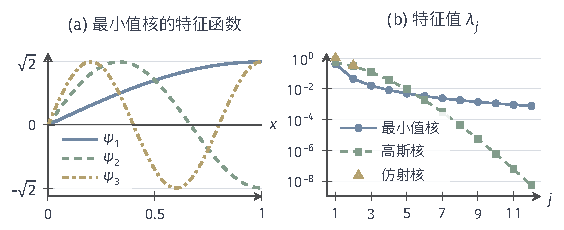
\includegraphics[width=95.5mm]{figures/02-abstract-mathematics/03-function-spaces/tikz/c5-mercer-spectrum/figure.pdf}
  \caption{Mercer特征函数与特征值衰减。(a)~最小值核在$[0,1]$、Lebesgue测度下的前三个特征函数$\psi_j=\sqrt2\sin((j-\frac12)\pi x)$，它们在$0$处为零、在$1$处导数为零；(b)~特征值（对数纵轴）：最小值核$\lambda_j=((j-\frac12)\pi)^{-2}$；高斯核（$\sigma=0.5$，$[-1,1]$，$\mathrm dz/2$）的特征值由40点Gauss--Legendre求积离散计算；仿射核只有$1$与$1/3$两个正特征值。}
  \label{fig:rkhs-mercer-spectrum}
\end{figure}

\subsection{核范数与谱系数}
\label{sec:rkhs-spectral-norm}

Mercer展开把核写成了特征映射$\Phi(x)=(\sqrt{\lambda_j}\psi_j(x))_j$的内积，这正好可以代入第~\ref{sec:rkhs-feature-maps}节的定理，读出核范数在谱坐标下的形式。

\paragraph{谱坐标下的核范数}

\begin{theorem}[核范数的谱表示]
\label{thm:rkhs-spectral-norm}
在定理~\ref{thm:rkhs-mercer}的条件下：
\begin{enumerate}
\item $\{\sqrt{\lambda_j}\,\psi_j\}$是$H_K$的标准正交基；
\item 函数$f:X\to\mathbb R$属于$H_K$，当且仅当存在实数列$(b_j)$满足$\sum_jb_j^2/\lambda_j<\infty$，且$f(x)=\sum_jb_j\psi_j(x)$对一切$x$成立。此时级数在$X$上绝对一致收敛，$b_j=\langle f,\psi_j\rangle_{L^2(\mu)}$，并且
\begin{equation}
\|f\|_{L^2(\mu)}^2=\sum_jb_j^2,\qquad \|f\|_{H_K}^2=\sum_j\frac{b_j^2}{\lambda_j}.
\label{eq:rkhs-two-norms}
\end{equation}
\end{enumerate}
\end{theorem}

\begin{proof}
令$\mathcal F=\ell^2$，$\Phi(x)=(\sqrt{\lambda_j}\psi_j(x))_j$。由定理~\ref{thm:rkhs-mercer}的第一步，$\|\Phi(x)\|^2=K(x,x)<\infty$；由Mercer展开，$\langle\Phi(x),\Phi(z)\rangle=K(x,z)$，所以$\Phi$是$K$的特征映射。先证可见子空间是整个$\ell^2$。设$w\in\ell^2$与每个$\Phi(x)$正交，即$\sum_jw_j\sqrt{\lambda_j}\psi_j(x)=0$对一切$x$成立。由于$\sqrt{\lambda_j}\le\sqrt{\lambda_1}$，系数$w_j\sqrt{\lambda_j}$平方可和，同一级数在$L^2(\mu)$中也收敛，其$L^2$极限与逐点极限几乎处处一致，因而为零；由$\psi_j$的标准正交性，$w_j\sqrt{\lambda_j}=0$，即$w=0$。

于是由定理~\ref{thm:rkhs-feature-space}，$w\mapsto f_w=\sum_jw_j\sqrt{\lambda_j}\psi_j$是从$\ell^2$到$H_K$的等距同构，单位向量$e_j$映为$\sqrt{\lambda_j}\psi_j$，这证明第1条。令$b_j=w_j\sqrt{\lambda_j}$，条件$w\in\ell^2$就是$\sum_jb_j^2/\lambda_j<\infty$，且$\|f_w\|_{H_K}^2=\sum_jw_j^2=\sum_jb_j^2/\lambda_j$。一致收敛来自
\[
\Bigl|\sum_{j>m}b_j\psi_j(x)\Bigr|\le\Bigl(\sum_{j>m}\frac{b_j^2}{\lambda_j}\Bigr)^{1/2}\Bigl(\sum_{j>m}\lambda_j\psi_j(x)^2\Bigr)^{1/2}\le M\Bigl(\sum_{j>m}\frac{b_j^2}{\lambda_j}\Bigr)^{1/2} .
\]
一致收敛的级数也在$L^2(\mu)$中收敛到同一函数，由标准正交性得$b_j=\langle f,\psi_j\rangle_{L^2}$与$\|f\|_{L^2}^2=\sum_jb_j^2$。
\end{proof}

\paragraph{两种范数的权重}

式~\eqref{eq:rkhs-two-norms}说明，同一组谱坐标$b_j$在两种范数中得到不同的权重：$L^2$范数对每个坐标一视同仁，核范数则把第$j$个坐标的平方放大$1/\lambda_j$倍。$L^2$中的单位方向$\psi_j$在$H_K$中的长度是$\lambda_j^{-1/2}$，$H_K$中真正的单位方向是$\sqrt{\lambda_j}\psi_j$。由于$\lambda_j\to0$，特征值小的方向在核范数中代价很高。

图~\ref{fig:rkhs-norm-weights}用最小值核说明这种差别。$f=\psi_1$与$g=\psi_1+0.1\psi_8$的图像几乎重合，$\|f-g\|_{L^2}=0.1$；但$\|f-g\|_{H_{\min}}=0.1\,\omega_8=0.1\times7.5\pi\approx2.36$，比$\|f\|_{H_{\min}}=\omega_1=\pi/2\approx1.57$还大。积分误差小并不意味着核范数误差小，核范数还计入了函数的振荡：对最小值核，$\|f\|_{H_{\min}}=\|f'\|_{L^2}$，$g$的高频小波纹带来很大的导数。

\begin{figure}[!htb]
  \centering
  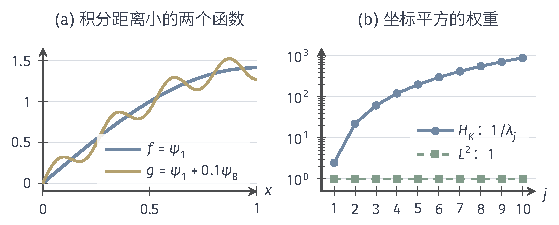
\includegraphics[width=94.6mm]{figures/02-abstract-mathematics/03-function-spaces/tikz/c5-norm-weights/figure.pdf}
  \caption{最小值核下两种范数的谱权重。(a)~$f=\psi_1$与$g=\psi_1+0.1\psi_8$，$\psi_j=\sqrt2\sin((j-\frac12)\pi x)$；两者的$L^2$距离为$0.1$，核范数距离却约为$2.36$。(b)~谱坐标平方在两种范数中的权重：$L^2$中恒为$1$，$H_K$中为$1/\lambda_j=((j-\frac12)\pi)^2$（对数纵轴），随$j$平方增长。}
  \label{fig:rkhs-norm-weights}
\end{figure}

\paragraph{哪些函数不在核空间中}

定理~\ref{thm:rkhs-spectral-norm}给出了$H_K$成员的两项要求：作为$L^2$元素，函数没有零谱分量；其谱坐标的加权平方和有限。两项要求可以分别不满足。在仿射核的例子中，$x^2=\tfrac13\psi_1+(x^2-\tfrac13)$含有零谱分量$x^2-\tfrac13$，所以不在$H_{\mathrm{aff}}$中，这一点也可以直接从$H_{\mathrm{aff}}$只含仿射函数看出。在最小值核的例子中零空间平凡，但常数函数$1$的谱坐标为$b_j=\int_0^1\sqrt2\sin(\omega_jx)\,\mathrm dx=\sqrt2/\omega_j$，于是$\sum_jb_j^2=\sum_j2/\omega_j^2=1=\|1\|_{L^2}^2$有限，而$\sum_jb_j^2/\lambda_j=\sum_j2$发散。常数$1$的谱展开在$L^2$中收敛，它却不属于$H_{\min}$，这与$H_{\min}$要求$f(0)=0$相符。

\paragraph{谱截断的两种尾和}

固定$f\in H_K$及其谱坐标$b_j$，令$f_m=\sum_{j\le m}b_j\psi_j$。由式~\eqref{eq:rkhs-two-norms}，
\begin{equation}
\|f-f_m\|_{L^2(\mu)}^2=\sum_{j>m}b_j^2\le\lambda_{m+1}\sum_{j>m}\frac{b_j^2}{\lambda_j}=\lambda_{m+1}\|f-f_m\|_{H_K}^2 ,
\label{eq:rkhs-tail-comparison}
\end{equation}
不等号用了$j>m$时$\lambda_j\le\lambda_{m+1}$。核范数尾和随$m\to\infty$趋于零，再由点值估计，
\[
|f(x)-f_m(x)|\le\sqrt{K(x,x)}\,\|f-f_m\|_{H_K}\le M\|f-f_m\|_{H_K},
\]
所以截断还一致收敛到$f$。逐点与一致控制来自核空间的点值有界性；一般的$L^2$正交展开没有这样的保证。式~\eqref{eq:rkhs-tail-comparison}还说明，对核范数不超过$R$的函数，$L^2$截断误差不超过$\sqrt{\lambda_{m+1}}R$，特征值衰减越快，这个统一的界越小。

以$H_{\min}$中的$f(x)=4x(1-x)$为例。它的谱坐标可以由分部积分算出：$b_j=4\sqrt2\bigl(2\omega_j^{-3}-(-1)^{j+1}\omega_j^{-2}\bigr)$，前三项约为$0.626,0.363,-0.068$；又$\|f\|_{L^2}^2=8/15$，$\|f\|_{H_{\min}}^2=\|f'\|_{L^2}^2=16/3$。取$m=3$，用总和减去前三项得$\|f-f_3\|_{L^2}\approx0.068$，$\|f-f_3\|_{H_{\min}}\approx1.07$。可以核对式~\eqref{eq:rkhs-tail-comparison}：$0.068^2\approx0.0046\le\lambda_4\times1.07^2\approx0.0083\times1.15\approx0.0095$。核范数尾和远大于$L^2$尾和，是因为$f'(1)=-4\ne0$而每个$\psi_j'(1)=0$，谱坐标只按$\omega_j^{-2}$衰减。

\paragraph{固定核而改变测度}

谱坐标依赖于测度，核范数却不依赖。仍取仿射核，把$[-1,1]$上的测度从$\mathrm dz/2$换成$\mathrm dz$，积分算子变为原来的两倍，特征值变为$2$与$2/3$，标准正交特征函数变为$1/\sqrt2$与$\sqrt{3/2}\,x$。对$f=a+bx$，新的谱坐标为$b_1=\sqrt2\,a$，$b_2=\int_{-1}^1(a+bx)\sqrt{3/2}\,x\,\mathrm dx=\sqrt{2/3}\,b$，于是
\[
\frac{b_1^2}{\lambda_1}+\frac{b_2^2}{\lambda_2}=\frac{2a^2}{2}+\frac{2b^2/3}{2/3}=a^2+b^2 ,
\]
与原来的核范数相同；而$L^2$范数平方从$a^2+b^2/3$变成了$2a^2+2b^2/3$。图~\ref{fig:rkhs-affine-norm-balls}在系数平面上画出三个单位球：核范数的单位球是圆，两个$L^2$单位球是形状不同的椭圆。这在一般情况下也成立：由定理~\ref{thm:rkhs-moore-aronszajn}，$H_K$的内积只由核决定；测度提供的是新的正交坐标和积分意义下的误差度量。

\begin{figure}[!htb]
  \centering
  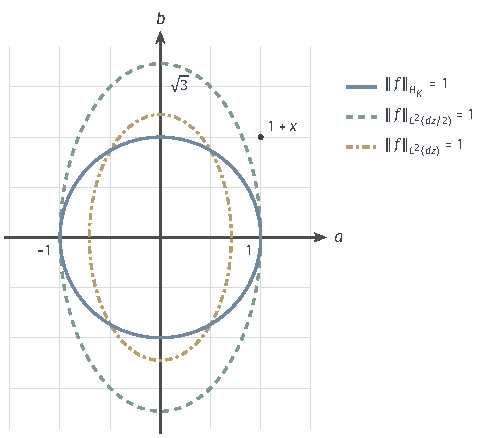
\includegraphics[width=82.4mm]{figures/02-abstract-mathematics/03-function-spaces/tikz/c5-affine-norm-balls/figure.pdf}
  \caption{仿射核$1+xz$在$[-1,1]$上，系数平面$(a,b)$（$f=a+bx$）中的三个单位球。实线圆是核范数单位球$a^2+b^2=1$，与测度无关；虚线椭圆是$L^2(\mathrm dz/2)$单位球$a^2+b^2/3=1$；点划线椭圆是$L^2(\mathrm dz)$单位球$2a^2+2b^2/3=1$。点$1+x$的核范数平方为$2$，$L^2(\mathrm dz/2)$范数平方为$4/3$。}
  \label{fig:rkhs-affine-norm-balls}
\end{figure}

\subsection{有限谱特征}
\label{sec:rkhs-finite-features}

上一小节截断的是一个给定函数的谱展开。本小节截断核本身，得到对所有函数同时适用的有限维表示，再与第~\ref{sec:rkhs-center-projection}节由观测中心得到的有限表示作比较。

\paragraph{谱特征与核近似}

保留前$m$个正谱方向，令
\[
\begin{aligned}
\Phi_m(x)&=\bigl(\sqrt{\lambda_1}\psi_1(x),\ldots,\sqrt{\lambda_m}\psi_m(x)\bigr)\in\mathbb R^m,\\
K_m(x,z)&=\Phi_m(x)^{\top}\Phi_m(z)=\sum_{j\le m}\lambda_j\psi_j(x)\psi_j(z).
\end{aligned}
\]
由定理~\ref{thm:rkhs-spectral-norm}，$K_m$是子空间$H_m=\operatorname{span}\{\psi_1,\ldots,\psi_m\}$（带$H_K$的内积）的再生核，$K-K_m$是其正交补的再生核。记对角余项$R_m(x)=K(x,x)-K_m(x,x)=\sum_{j>m}\lambda_j\psi_j(x)^2\ge0$，由Cauchy--Schwarz不等式，
\begin{equation}
|K(x,z)-K_m(x,z)|\le\sqrt{R_m(x)R_m(z)},\qquad
\int_XR_m\,\mathrm d\mu=\sum_{j>m}\lambda_j .
\label{eq:rkhs-kernel-truncation}
\end{equation}
Mercer定理保证$\max_xR_m(x)\to0$，所以$K_m$在$X\times X$上一致逼近$K$；积分意义下的误差恰好是特征值的尾和。对最小值核取$m=3$，$\int_0^1R_3\,\mathrm dx=\tfrac12-\sum_{j\le3}\omega_j^{-2}\approx0.0335$，$\max R_3\approx0.067$。

\paragraph{核误差与函数误差}

核误差与函数误差是两个不同的量。$f-f_m$属于$H_m$的正交补，而它的再生核是$K-K_m$，所以
\begin{equation}
|f(x)-f_m(x)|=\bigl|\langle f-f_m,(K-K_m)_x\rangle_{H_K}\bigr|\le\sqrt{R_m(x)}\,\|f-f_m\|_{H_K}.
\label{eq:rkhs-spectral-pointwise}
\end{equation}
右端的第一个因子只依赖于核与测度，第二个因子取决于$f$的谱坐标尾和。核误差小说明所有函数在单位核范数意义下被同时控制；某个具体函数的误差还取决于它的高频坐标有多大。另外，$f_m$既是$f$在$H_m$上的$L^2(\mu)$正交投影，也是$H_K$正交投影，因为$\psi_j$在两种内积下都两两正交。

\paragraph{谱截断与中心投影}

式~\eqref{eq:rkhs-spectral-pointwise}与第~\ref{sec:rkhs-center-projection}节的式~\eqref{eq:rkhs-power-bound}有完全相同的结构：一个$m$维子空间，它的再生核把余项的对角值留给误差界。两者的区别在于子空间由什么信息决定。中心投影的$M_Z$由观测位置决定，不需要测度，只需核值与读数；谱截断的$H_m$由测度下积分算子的特征函数决定，需要先求解积分算子的特征问题。

图~\ref{fig:rkhs-truncation-comparison}在最小值核上比较两者，都取三维：谱截断取$m=3$，中心投影取$Z=\{1/3,2/3,1\}$（第~\ref{sec:rkhs-center-projection}节已算出它是折线插值）。对核本身，中心投影的对角余项$P_Z^2$在中心处为零，但积分为$1/18\approx0.056$、最大值$1/12\approx0.083$，都大于谱截断的$0.0335$与$0.067$。对目标$f=4x(1-x)$，谱截断的$L^2$误差约$0.068$，小于中心投影的$0.081$；但中心投影的核范数误差约$0.77$、最大逐点误差约$0.11$，分别小于谱截断的$1.07$与$0.28$。谱截断在$x=1$附近误差最大，因为所有$\psi_j$在那里导数为零，而中心投影在$1$处恰好有一个观测。哪一种更好，取决于所用的误差度量，两种有限表示保留的是不同的子空间。

\begin{figure}[!htb]
  \centering
  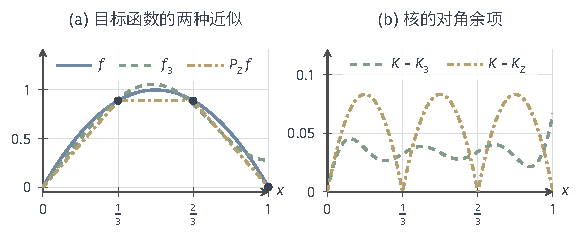
\includegraphics[width=98.2mm]{figures/02-abstract-mathematics/03-function-spaces/tikz/c5-truncation-comparison/figure.pdf}
  \caption{最小值核（$[0,1]$，Lebesgue测度）下三维谱截断与三个中心$Z=\{1/3,2/3,1\}$的投影。(a)~目标$f=4x(1-x)$（实线）、谱截断$f_3$（虚线）与中心投影$P_Zf$（点划线，即过黑点的折线）；(b)~核的对角余项$R_3(x)=K(x,x)-K_3(x,x)$与$P_Z(x)^2=K(x,x)-K_Z(x,x)$，后者在中心处为零但积分更大。}
  \label{fig:rkhs-truncation-comparison}
\end{figure}

在实际计算中，测度常常未知或只能通过样本给出，积分算子的特征函数也无法精确求得。由样本点构造核矩阵并取其谱分解，得到的正是第~\ref{sec:rkhs-center-projection}节的投影核$K_Z$及其有限特征$\Phi_Z$，而不是这里的$K_m$。样本中心与积分谱之间的关系、随机抽取中心或随机特征时的误差，需要另外引入抽样模型来分析；本节的尾和结论不能自动搬到这些数值方法上。
